\documentclass[12pt]{article}
\usepackage[italian]{babel}
\usepackage{geometry}
\usepackage{amsmath}
\usepackage{amssymb}
\usepackage{graphicx}
\usepackage{ulem}

\geometry{margin=2cm}
\let\olditemize\itemize
\renewcommand\itemize{\olditemize\setlength\itemsep{0em}}

\title{Gestore delle strutture di memorizzazione}
\author{Lorenzo Vaccarecci}
\date{8 Marzo 2024}

\graphicspath{{../Immagini/}}

\begin{document}
\maketitle
\section{Gerarchia delle memorie}
\begin{itemize}
    \item Prestazioni di una memoria: tempo di accesso ottenuto dalla somma di \begin{itemize}
        \item Latenza: tempo necessario per accedere al primo byte di interesse
        \item Tempo di trasferimento: tempo necessario per spostare i dati tra livelli della gerarchia 
    \end{itemize}
\end{itemize}
\begin{equation*}
    \text{Tempo di accesso} = \text{Latenza} + \frac{\text{dimensione dati da trasferire}}{\text{velocità di trasferimento}}
\end{equation*}
La gerarchia può essere vista come una piramide, i dischi saranno in basso (lento, economica e grande) mentre la \textbf{memoria principale} sarà in alto (veloce, costosa, piccola).
% Perchè i dischi sono lenti
% Come si può rappresentare BD a livello fisico
\section{Gestore dei file}
\subsection{Dischi magnetici}
\begin{description}
    \item[Cilindro]: è la porzione di disco che si trova ad una stessa distanza dal centro (la "riga" del disco). 
\end{description}
\textbf{Se i dati sono memorizzati su uno stesso cilindro (anche di tracce diverse) possono essere recuperati molto più velocemente che non dati distribuiti su diversi cilindri (il movimento della testina è molto lento).}
\begin{center}
    \begin{tabular}{| c | c | c |}
        \hline
        \textbf{Component} & \textbf{Best Case} & \textbf{Worst Case} \\ 
        \hline
        Command Overhead & 0.5 & 0.5 \\ % tempo impiegato a impartire comandi al drive
        \hline
        Seek Time & 2.2 & 15.5 \\ % tempo impiegato dal braccio a posizionarsi sulla traccia desiderata
        \hline
        Settle Time & $<$0.1 & $<$0.1 \\ % tempo impiegato per la stabilizzazione del braccio
        \hline
        Rotational Latency & 0.0 & 8.3 \\ % tempo di attesa dal primo settore da leggere
        \hline
        Total & 2.7 & 28.4 \\
        \hline
    \end{tabular}    
\end{center}
\begin{description}
    \item[Command Overhead]: tempo impiegato a impartire comandi al drive
    \item[Seek Time]: tempo impiegato dal braccio a posizionarsi sulla traccia desiderata
    \item[Settle Time]: tempo impiegato per la stabilizzazione del braccio
    \item[Rotational Latency]: tempo di attesa dal primo settore da leggere
\end{description}
\subsubsection{Tempo di trasferimento}
\begin{itemize}
    \item Tempo per trasferire un certo numero di byte
    \item Si riferisce alla velocità con cui si trasferiscono byte dai (sui) piatti sulla (dalla) cache del controller
    \item Dipende dalla \textbf{velocità di trasferimento (o transfer rate $Tr$): numero di byte trasferiti nell'unità di tempo} \begin{itemize}
    \item Si può dimostrare come: (dim dati su una traccia) / tempo di rotazione
    \item Tipicamente dell'ordine di qualche decina di MB/sec
    \end{itemize}
\end{itemize}
Un blocco (o pagina) è una sequenza contigua di settori su una traccia, e costituisce l'unità di I/o per il trasferimento dei dati tra il disco e la memoria principale.
\begin{itemize}
    \item Il tempo di latenza: quale decina di msec nel caso peggiore.
    \item Il tempo di trasferimento: circa 1msec per blocchi da 4KB.
    \item \textbf{Il gestore delle strutture di memorizzazione deve cercare di ridurre il tempo di latenza.}
\end{itemize}
\subsection{Il DB Fisico}
\begin{itemize}
    \item \textbf{A livello fisico di un DB consiste di un insieme di file, ognuno di quali viene visto come una collezione di pagine, di dimensione fissa}
    \item Ogni pagina/blocco memorizza più \textbf{record} (corrispondenti alle tuple logiche)
\end{itemize}
\begin{center}
    \begin{tabular}{| c | c |}
        \hline
        \textbf{LIVELLO LOGICO} & \textbf{LIVELLO FISICO} \\
        \hline
        Relazione (tabella) & File \\
        \hline
        Tupla & Record \\
        \hline
    \end{tabular}
\end{center}
\subsubsection{File}
\begin{itemize}
    \item un \textbf{file} è una sequenza di record
    \item un file è detto \textbf{file con record a lunghezza fissa} se tutti i record hanno la stessa dimensione (in byte)
    \item altrimenti parliamo di un \textbf{file con record a lunghezza variabile}
\end{itemize}
\subsubsection{Record}
    \textbf{Header} 
    \begin{itemize}
        \item L'identificatore della Relazione
        \item L'identificatore univoco RID
        \item timestamp
    \end{itemize}
\section{Allocazione dei file}
\begin{itemize}
    \item \textbf{Allocazione continua}: \begin{itemize}
        \item I blocchi dei file sono allocati in blocchi di disco contigui quindi non devo muovere troppo la testina
        \item Rende molto efficiente le letture dell'intero file
        \item Gli aggiornamenti sono costosi (se ho un file pieno e voglio aggiungere un record, devo spostare tutti i blocchi in un'altra posizione di lunghezza + 1)
    \end{itemize}
    \item \textbf{Allocazione concatenata}: \begin{itemize}
        \item Ogni blocco di un file contiene un puntatore al successivo blocco del file
        \item Gli aggiornamenti sono molto efficienti
        \item Lettura dell'intero file  molto lenta
        \item Utilizzo di \textbf{bucket} non necessariamente contigui ma vicini (possibilmente nello stesso cilindro), per gruppi di record tra loro collegati
    \end{itemize}
\end{itemize}
\section{Organizzazione dei record nei file}
\begin{itemize}
    \item \textbf{File heap}: i record vengono memorizzati in ordine di inserimento
    \item \textbf{File ordinato su $X$}: i record vengono memorizzati in ordine rispetto ad un campo $X$ 
    \item \textbf{File hash su $X$}: i record vengono memorizzati in ordine parziale rispetto ad un campo $X$ (vengono raggruppati in base al valore di $X$)
\end{itemize}
\begin{center}
    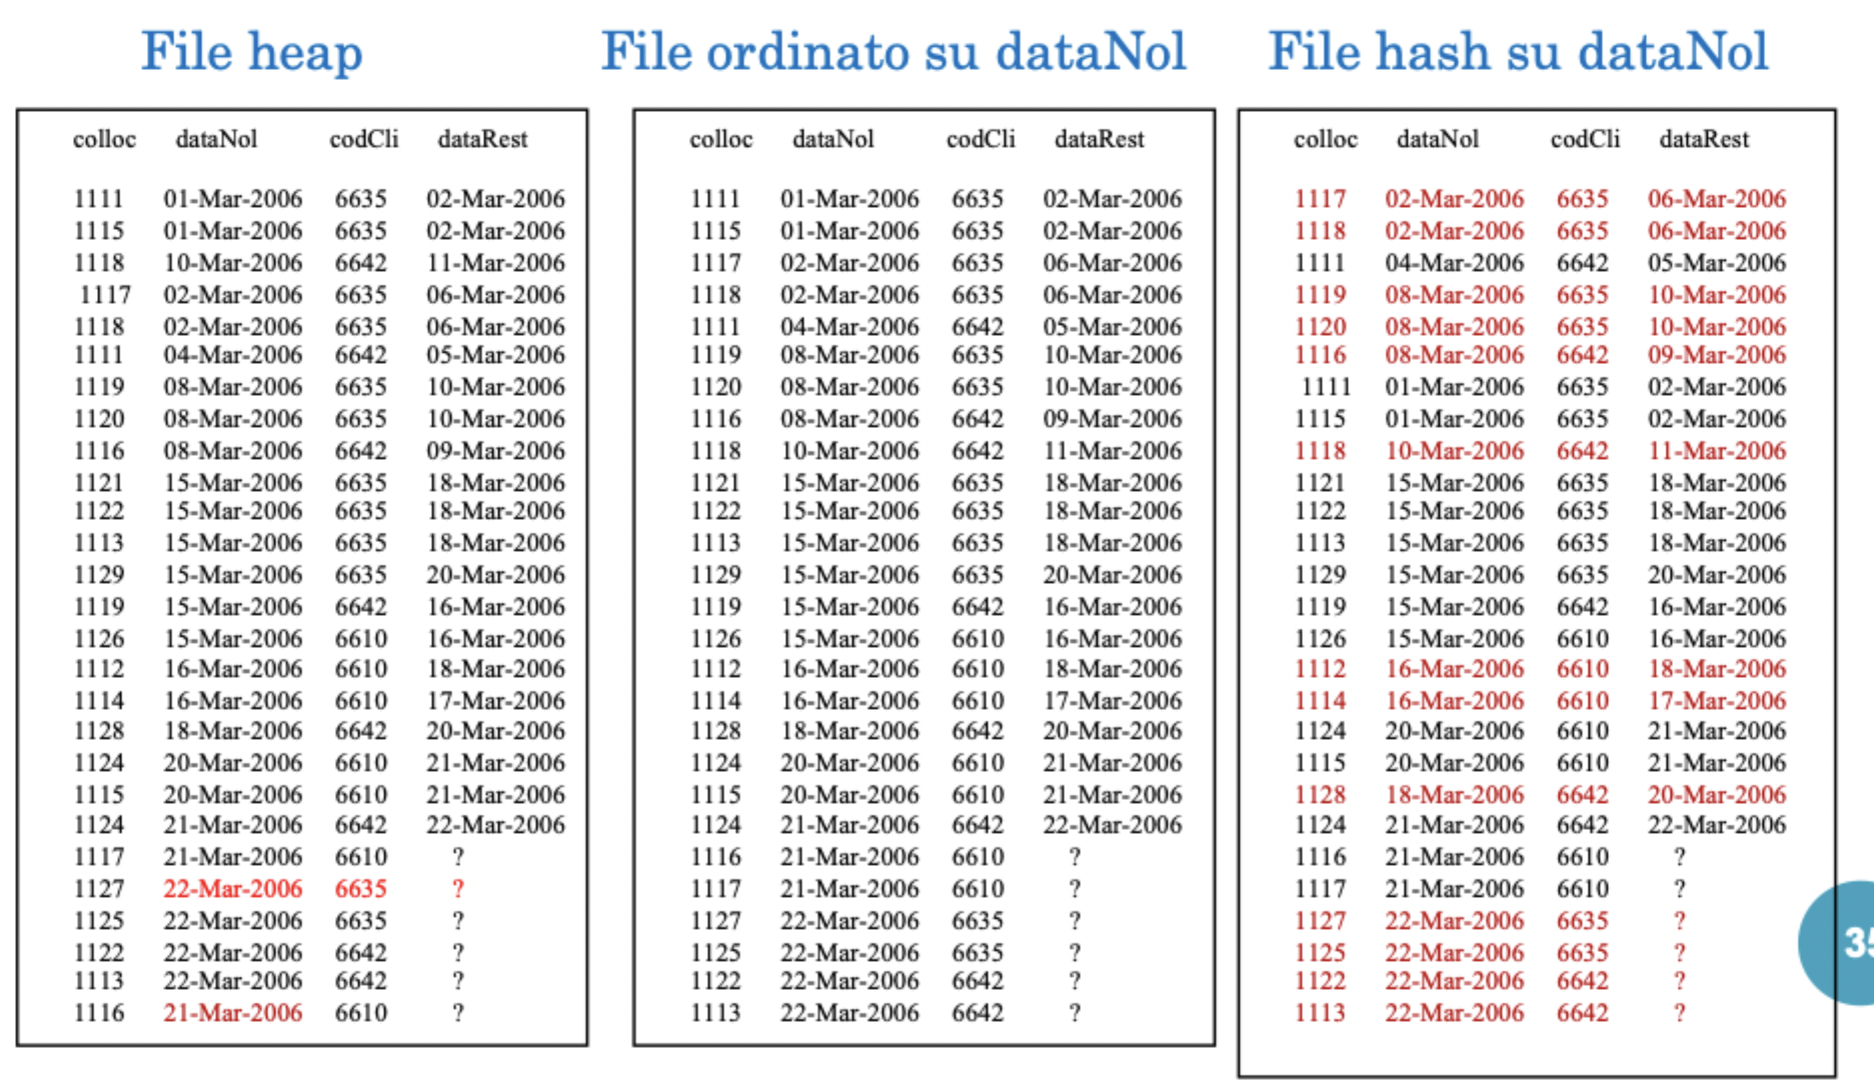
\includegraphics[width=\textwidth]{recordfile.png}
\end{center}
\end{document}